\section{Flashback} \label{sec:appendix:flashback}

\vfill
\begin{figure}[H]
  \center
  ing
  \includegraphics[height=.4\textheight]{img/pics/9.jpg}
  \caption{Early prototyping in 2024.}
  \label{fig:prototype1}  
\end{figure}
\vfill
\begin{figure}[H]
  \centering
  \includegraphics[height=.4\textheight]{img/pics/10.jpg}
  \caption{Early prototyping in 2024.}
  \label{fig:prototype2}
\end{figure}
\vfill

\newpage

\vfill
\begin{figure}[H]
  \centering
  \includegraphics[height=.4\textheight]{img/pics/11.jpg}
  \caption{Early prototyping in 2024.}
  \label{fig:prototype1}
\end{figure}
\vfill
\begin{figure}[H]
  \centering
  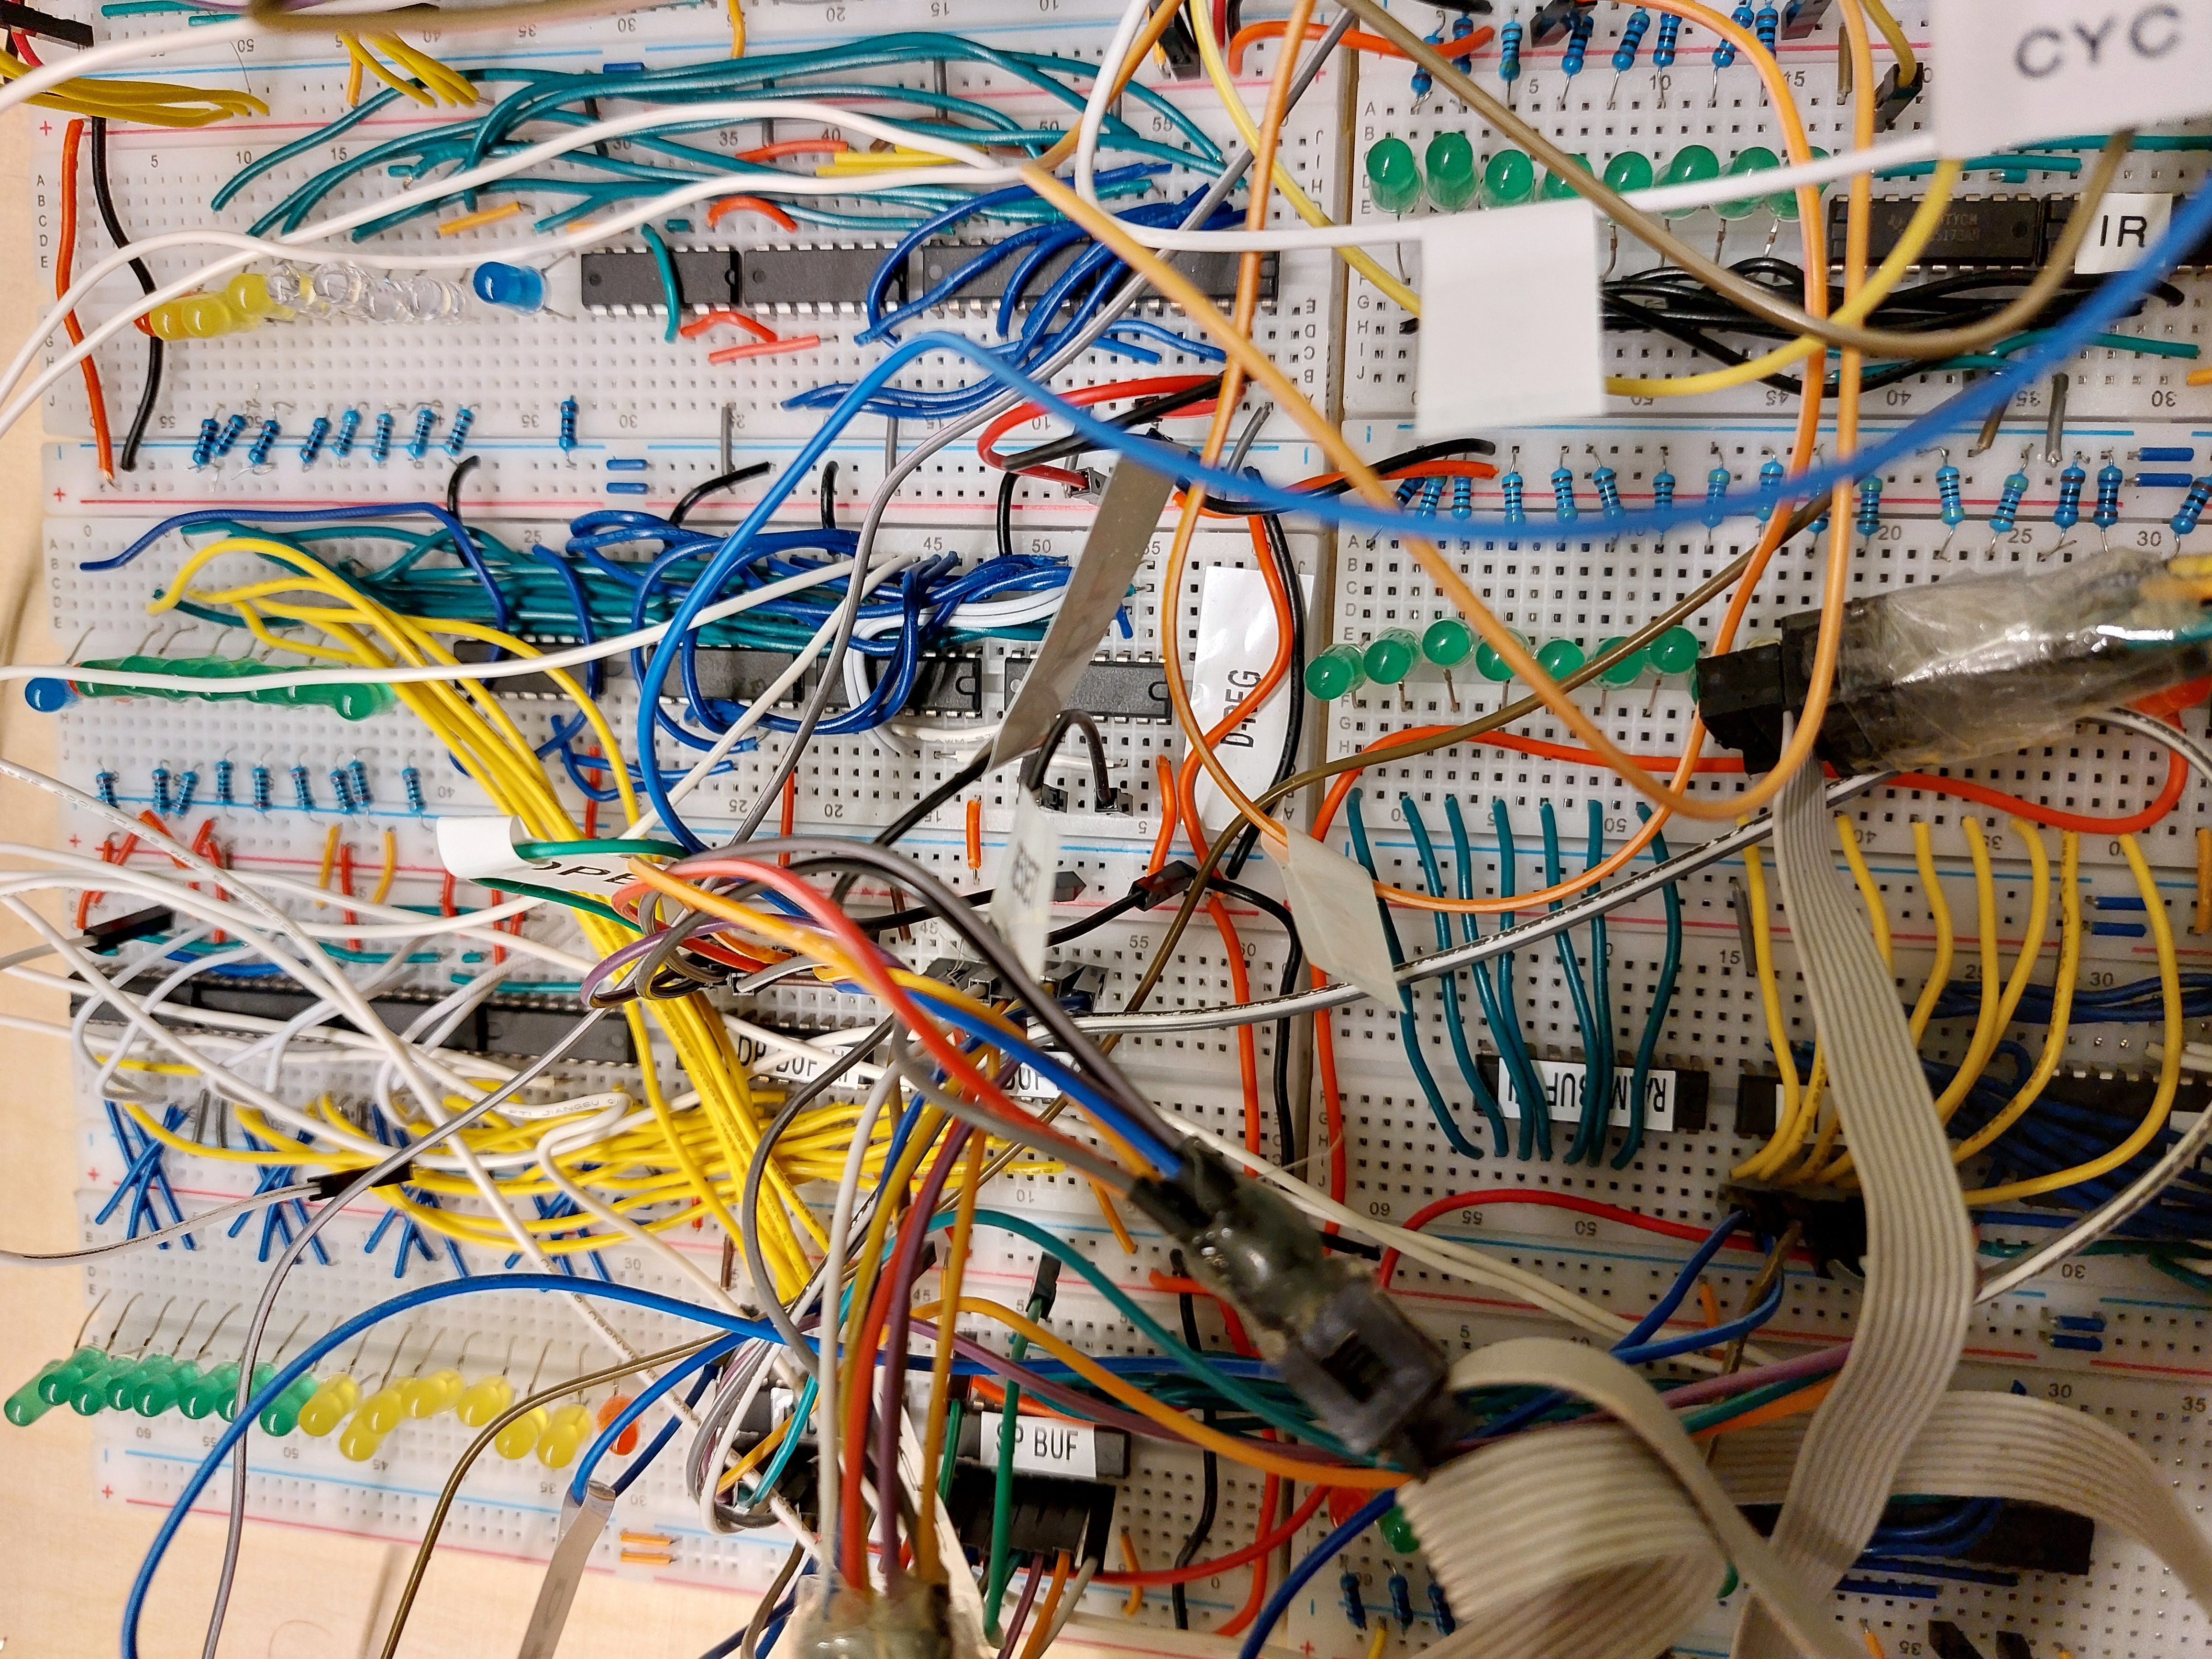
\includegraphics[height=.4\textheight]{img/pics/20241213_210401.jpg}
  \caption{Early prototyping in 2024.}
  \label{fig:messy1}
\end{figure}
\vfill

\newpage

\vfill
\begin{figure}[H]
  \centering
  \includegraphics[width=\textwidth]{img/pics/IMG-20250208-WA0007.jpeg}
  \caption{Wire stripping can quickly lead to a mess.}  
  \label{fig:messy2}
\end{figure}
\vfill
\begin{figure}[H]
  \centering
  \includegraphics[width=\textwidth]{img/pics/IMG-20250208-WA0010.jpeg}
  \caption{A typical view when building and debugging the system.}
  \label{fig:earlybuild1}
\end{figure}
\vfill

\newpage

\vfill
\begin{figure}[H]
  \centering
  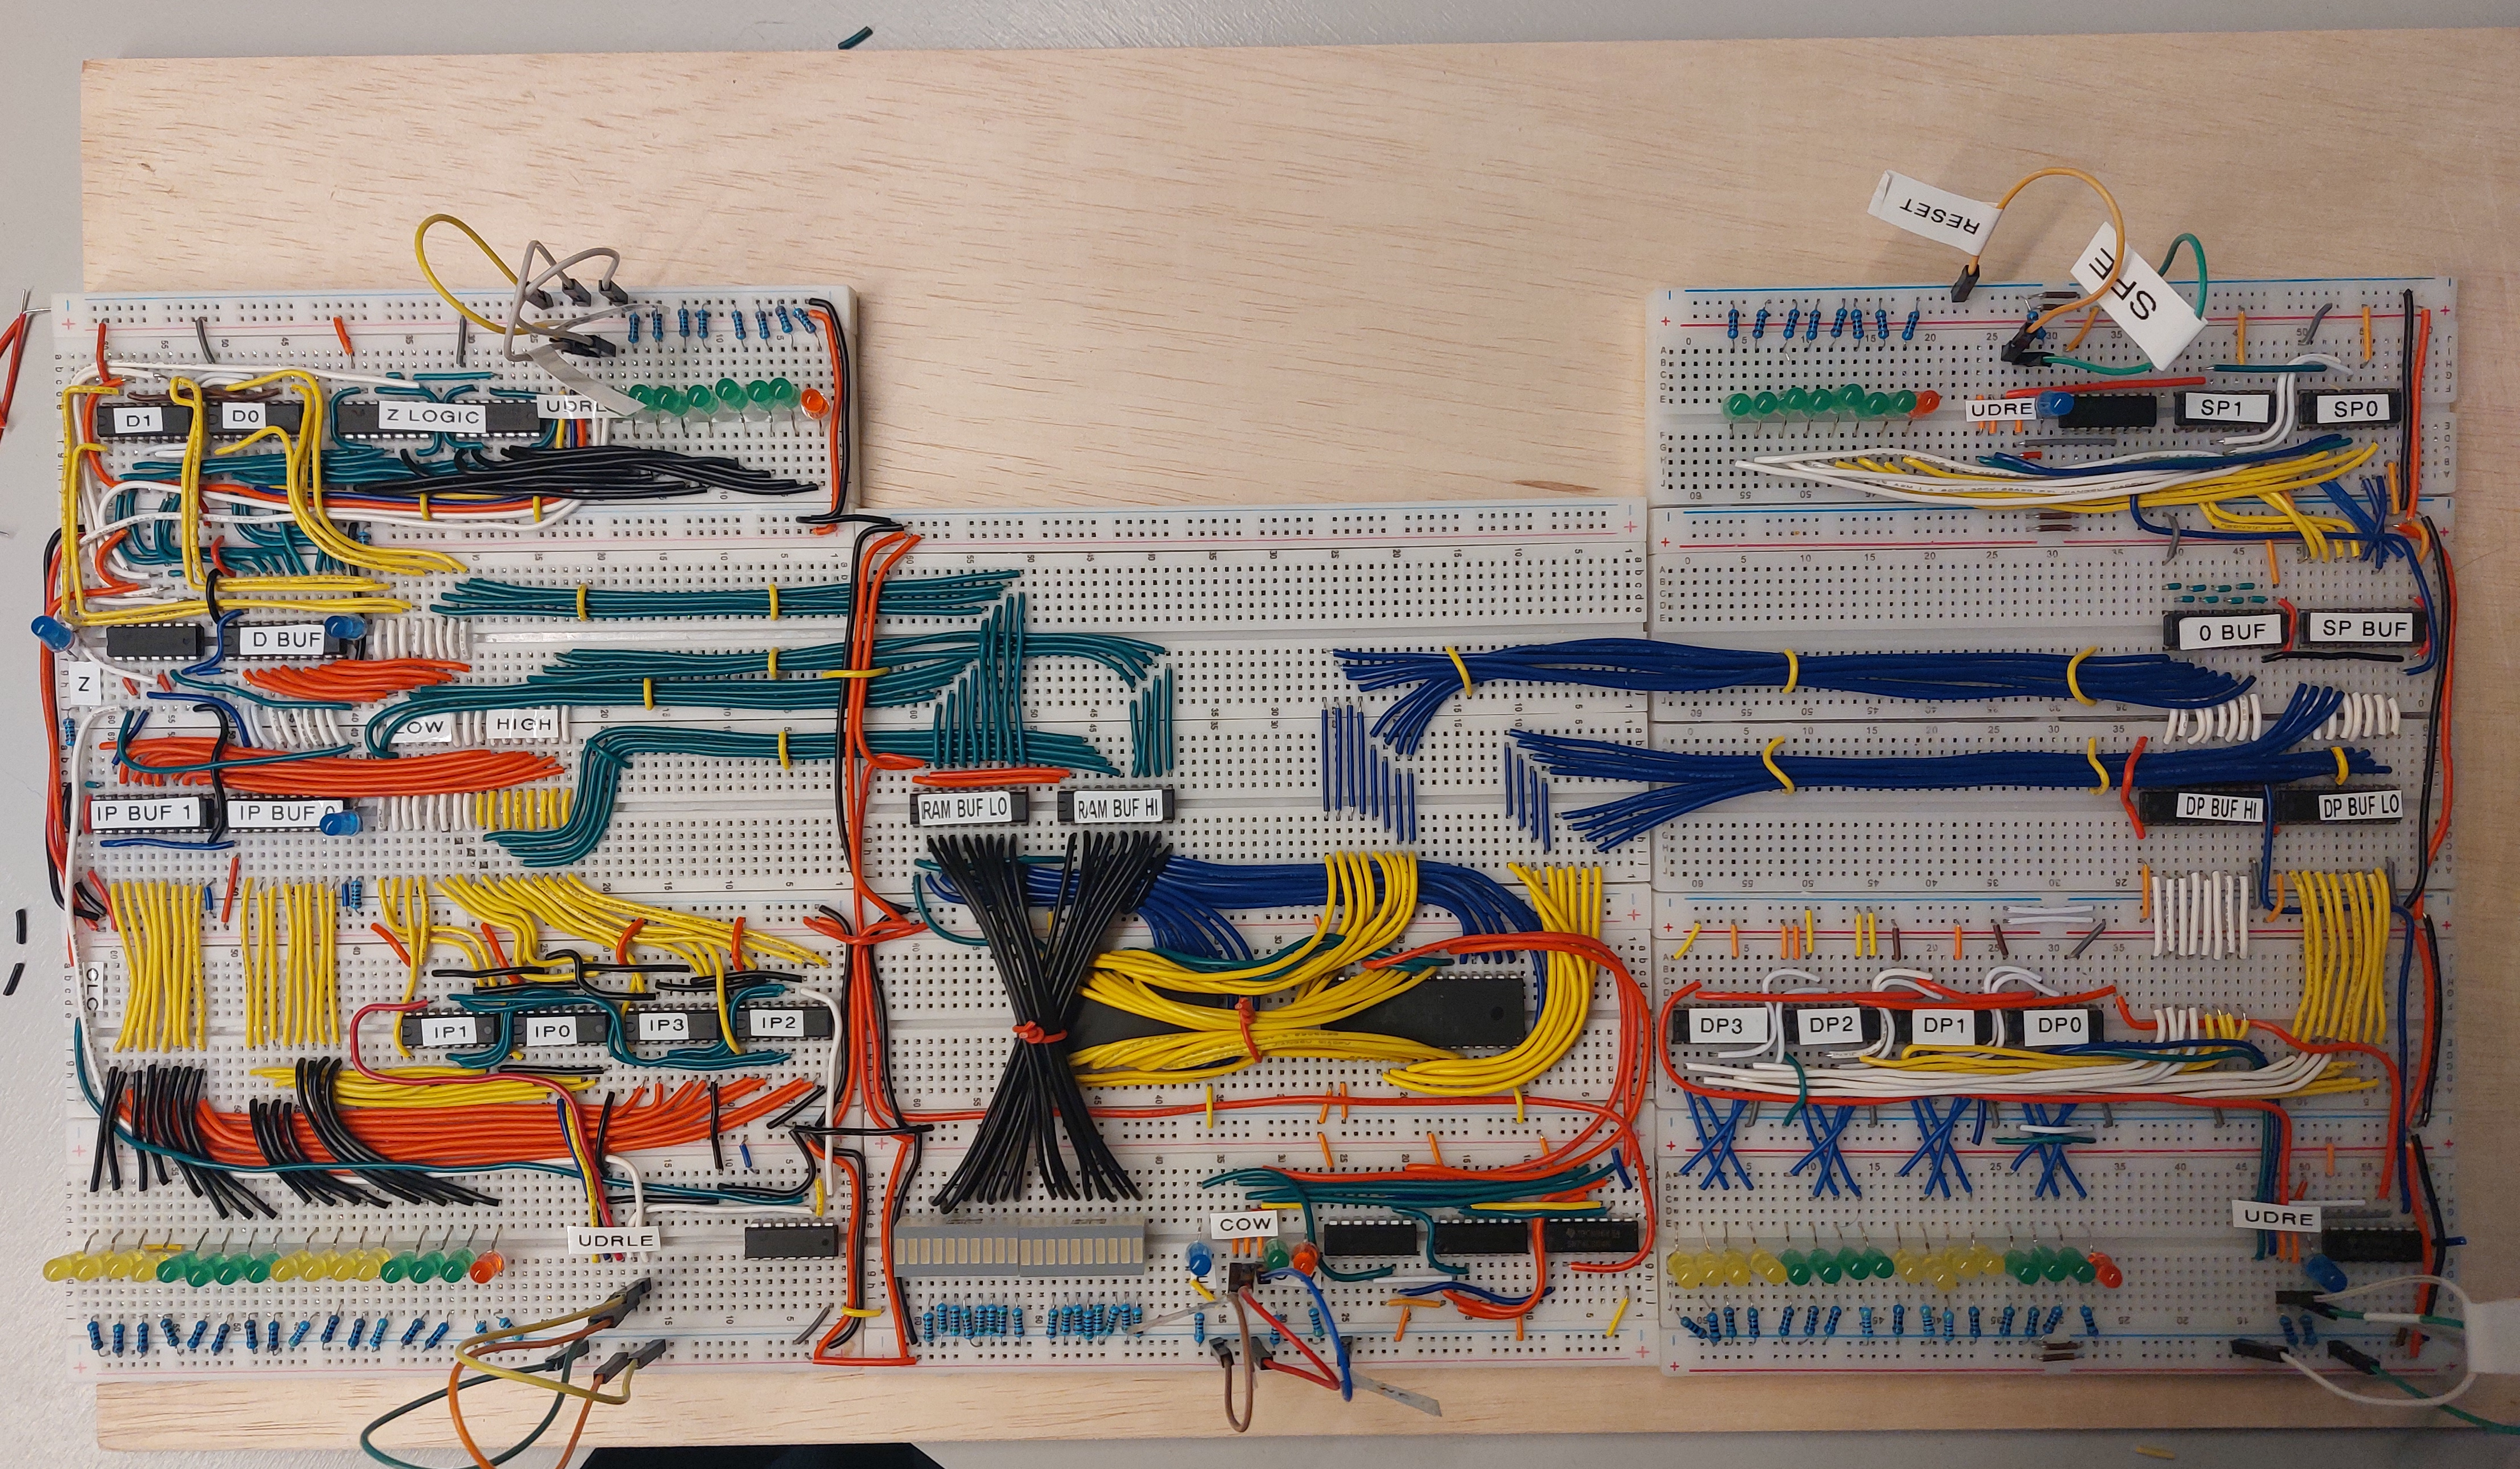
\includegraphics[width=.9\textwidth]{img/pics/20241222_141304.jpg}
  \caption{Registers and RAM first put together, the system starts to take shape.}  
  \label{fig:earlybuild2}    
\end{figure}
\vfill
\begin{figure}[H]
  \centering
  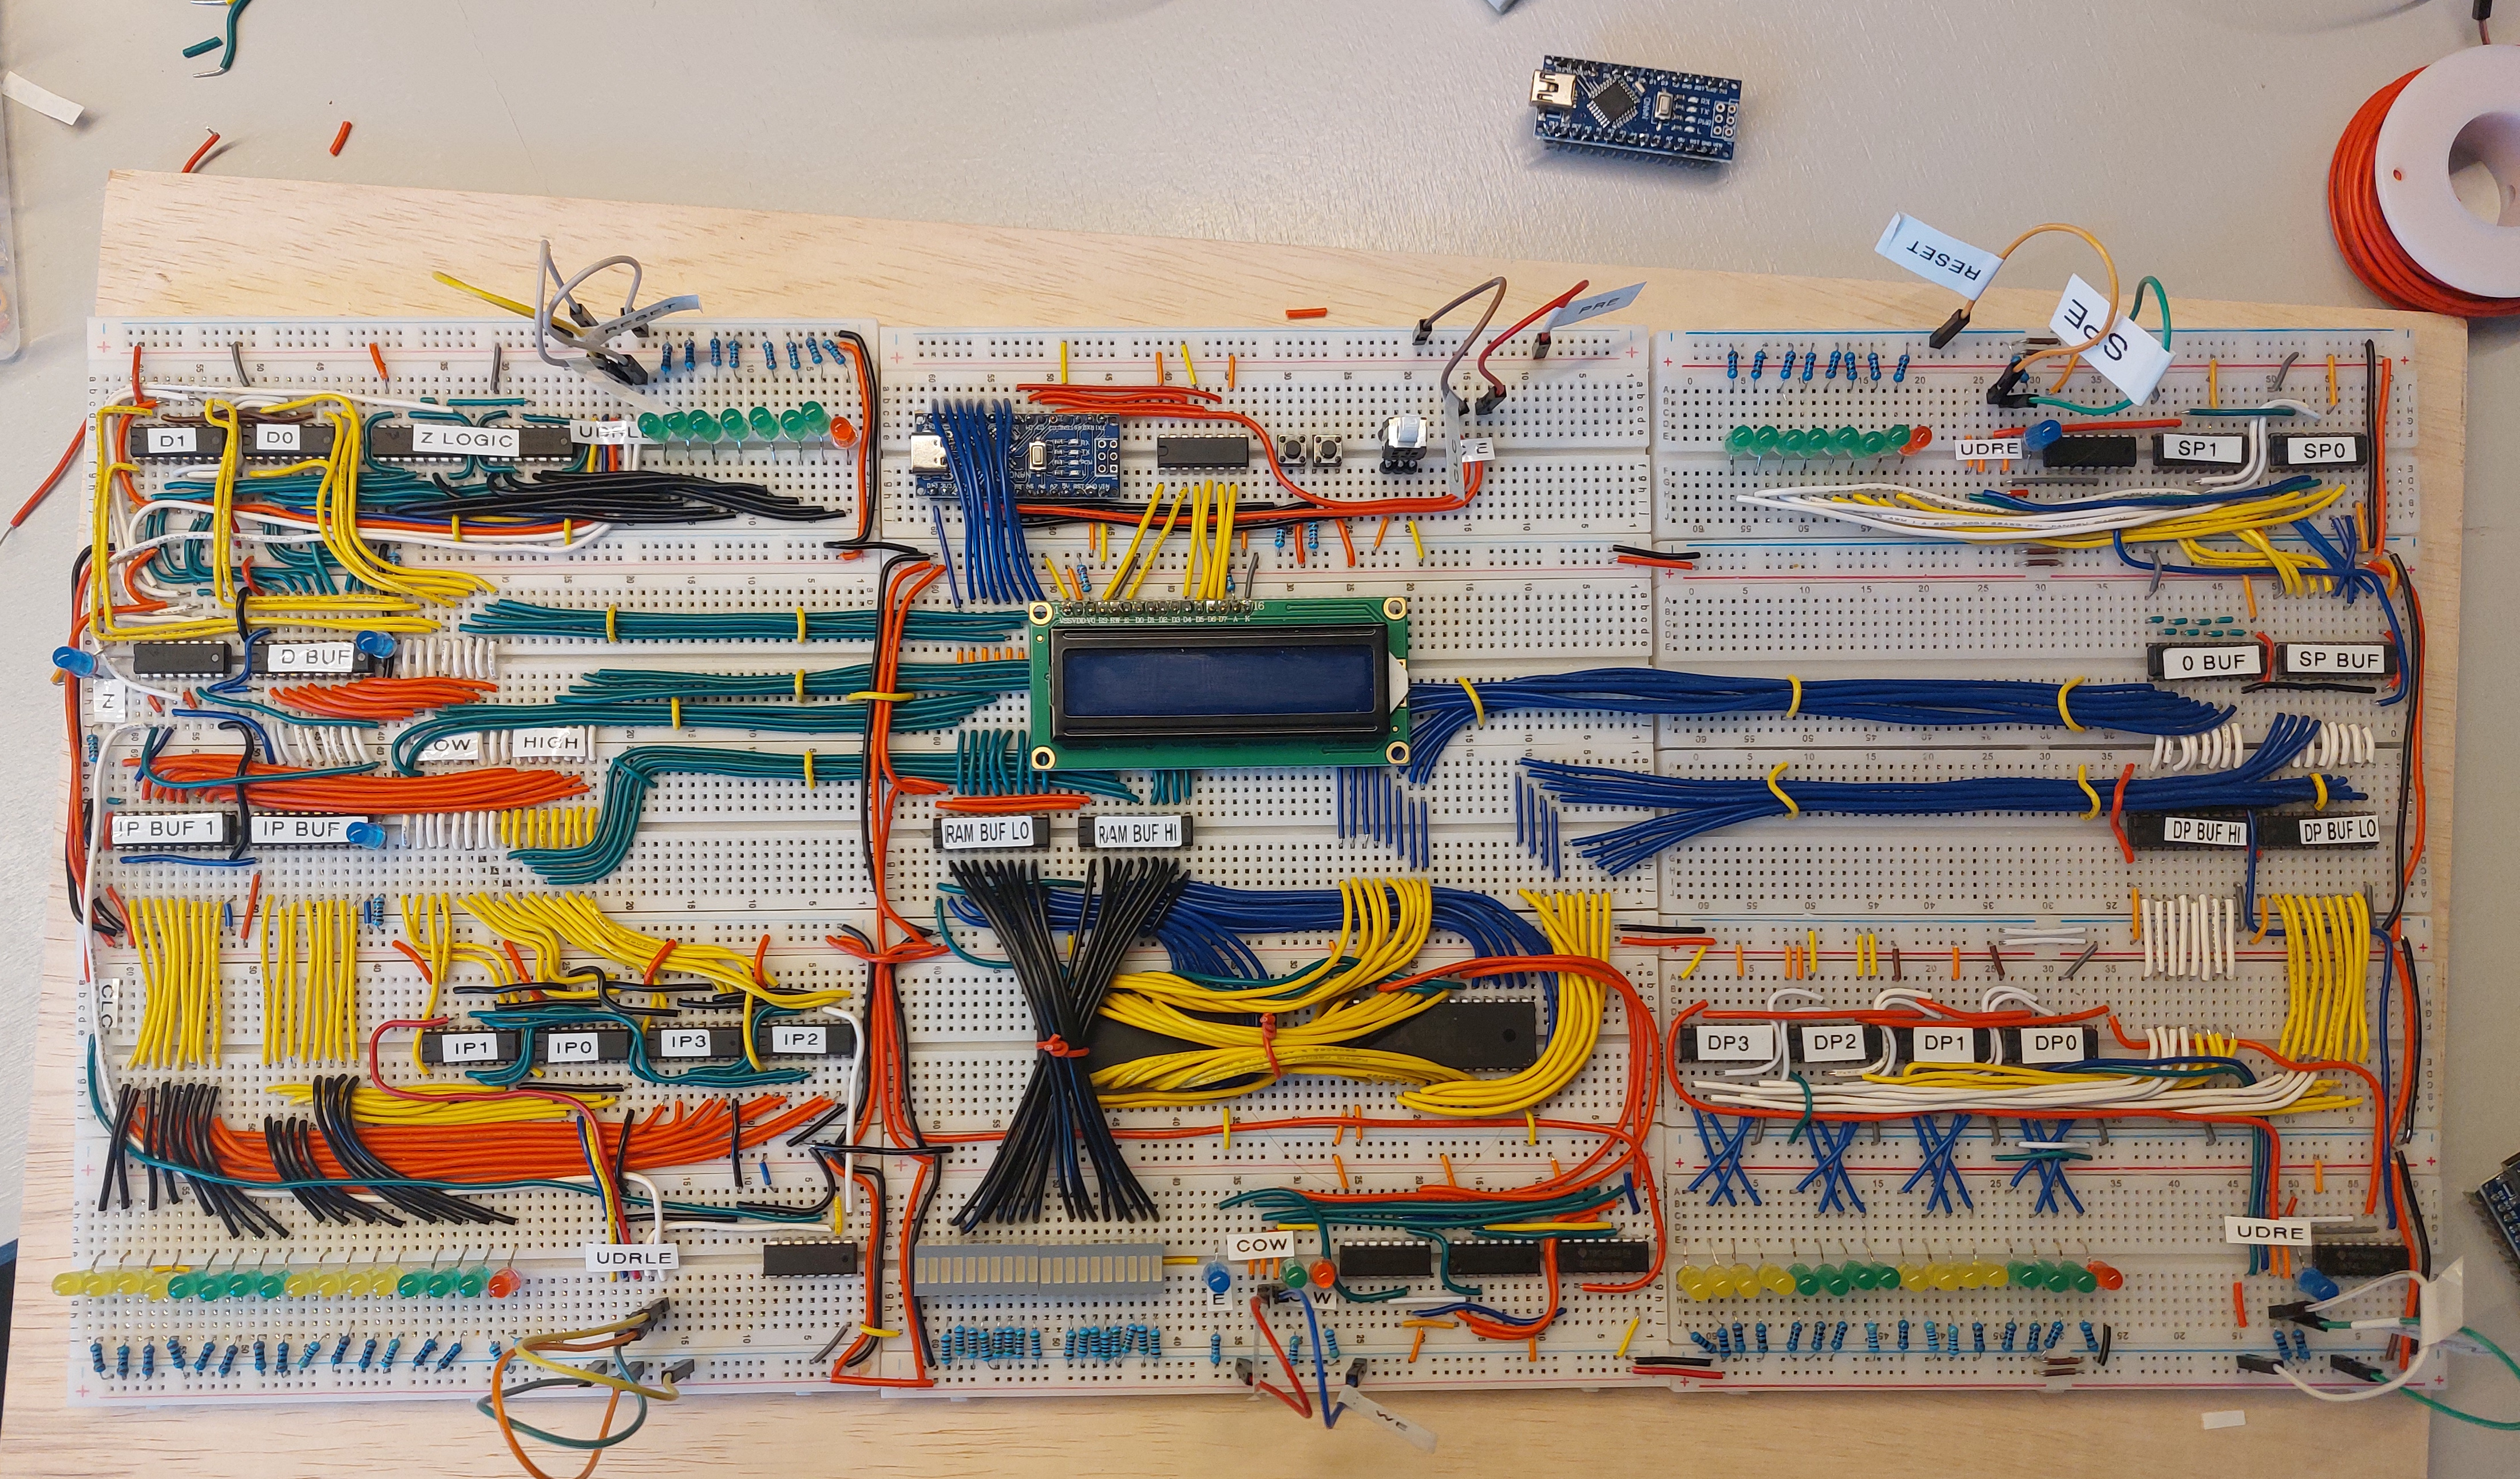
\includegraphics[width=.9\textwidth]{img/pics/20241223_134527.jpg}
  \caption{An early version of the IO module, including an Arduino Nano, was added to the system.}
  \label{fig:earlybuild3}
\end{figure}
\vfill

\newpage

\vfill
\begin{figure}[H]
  \centering
  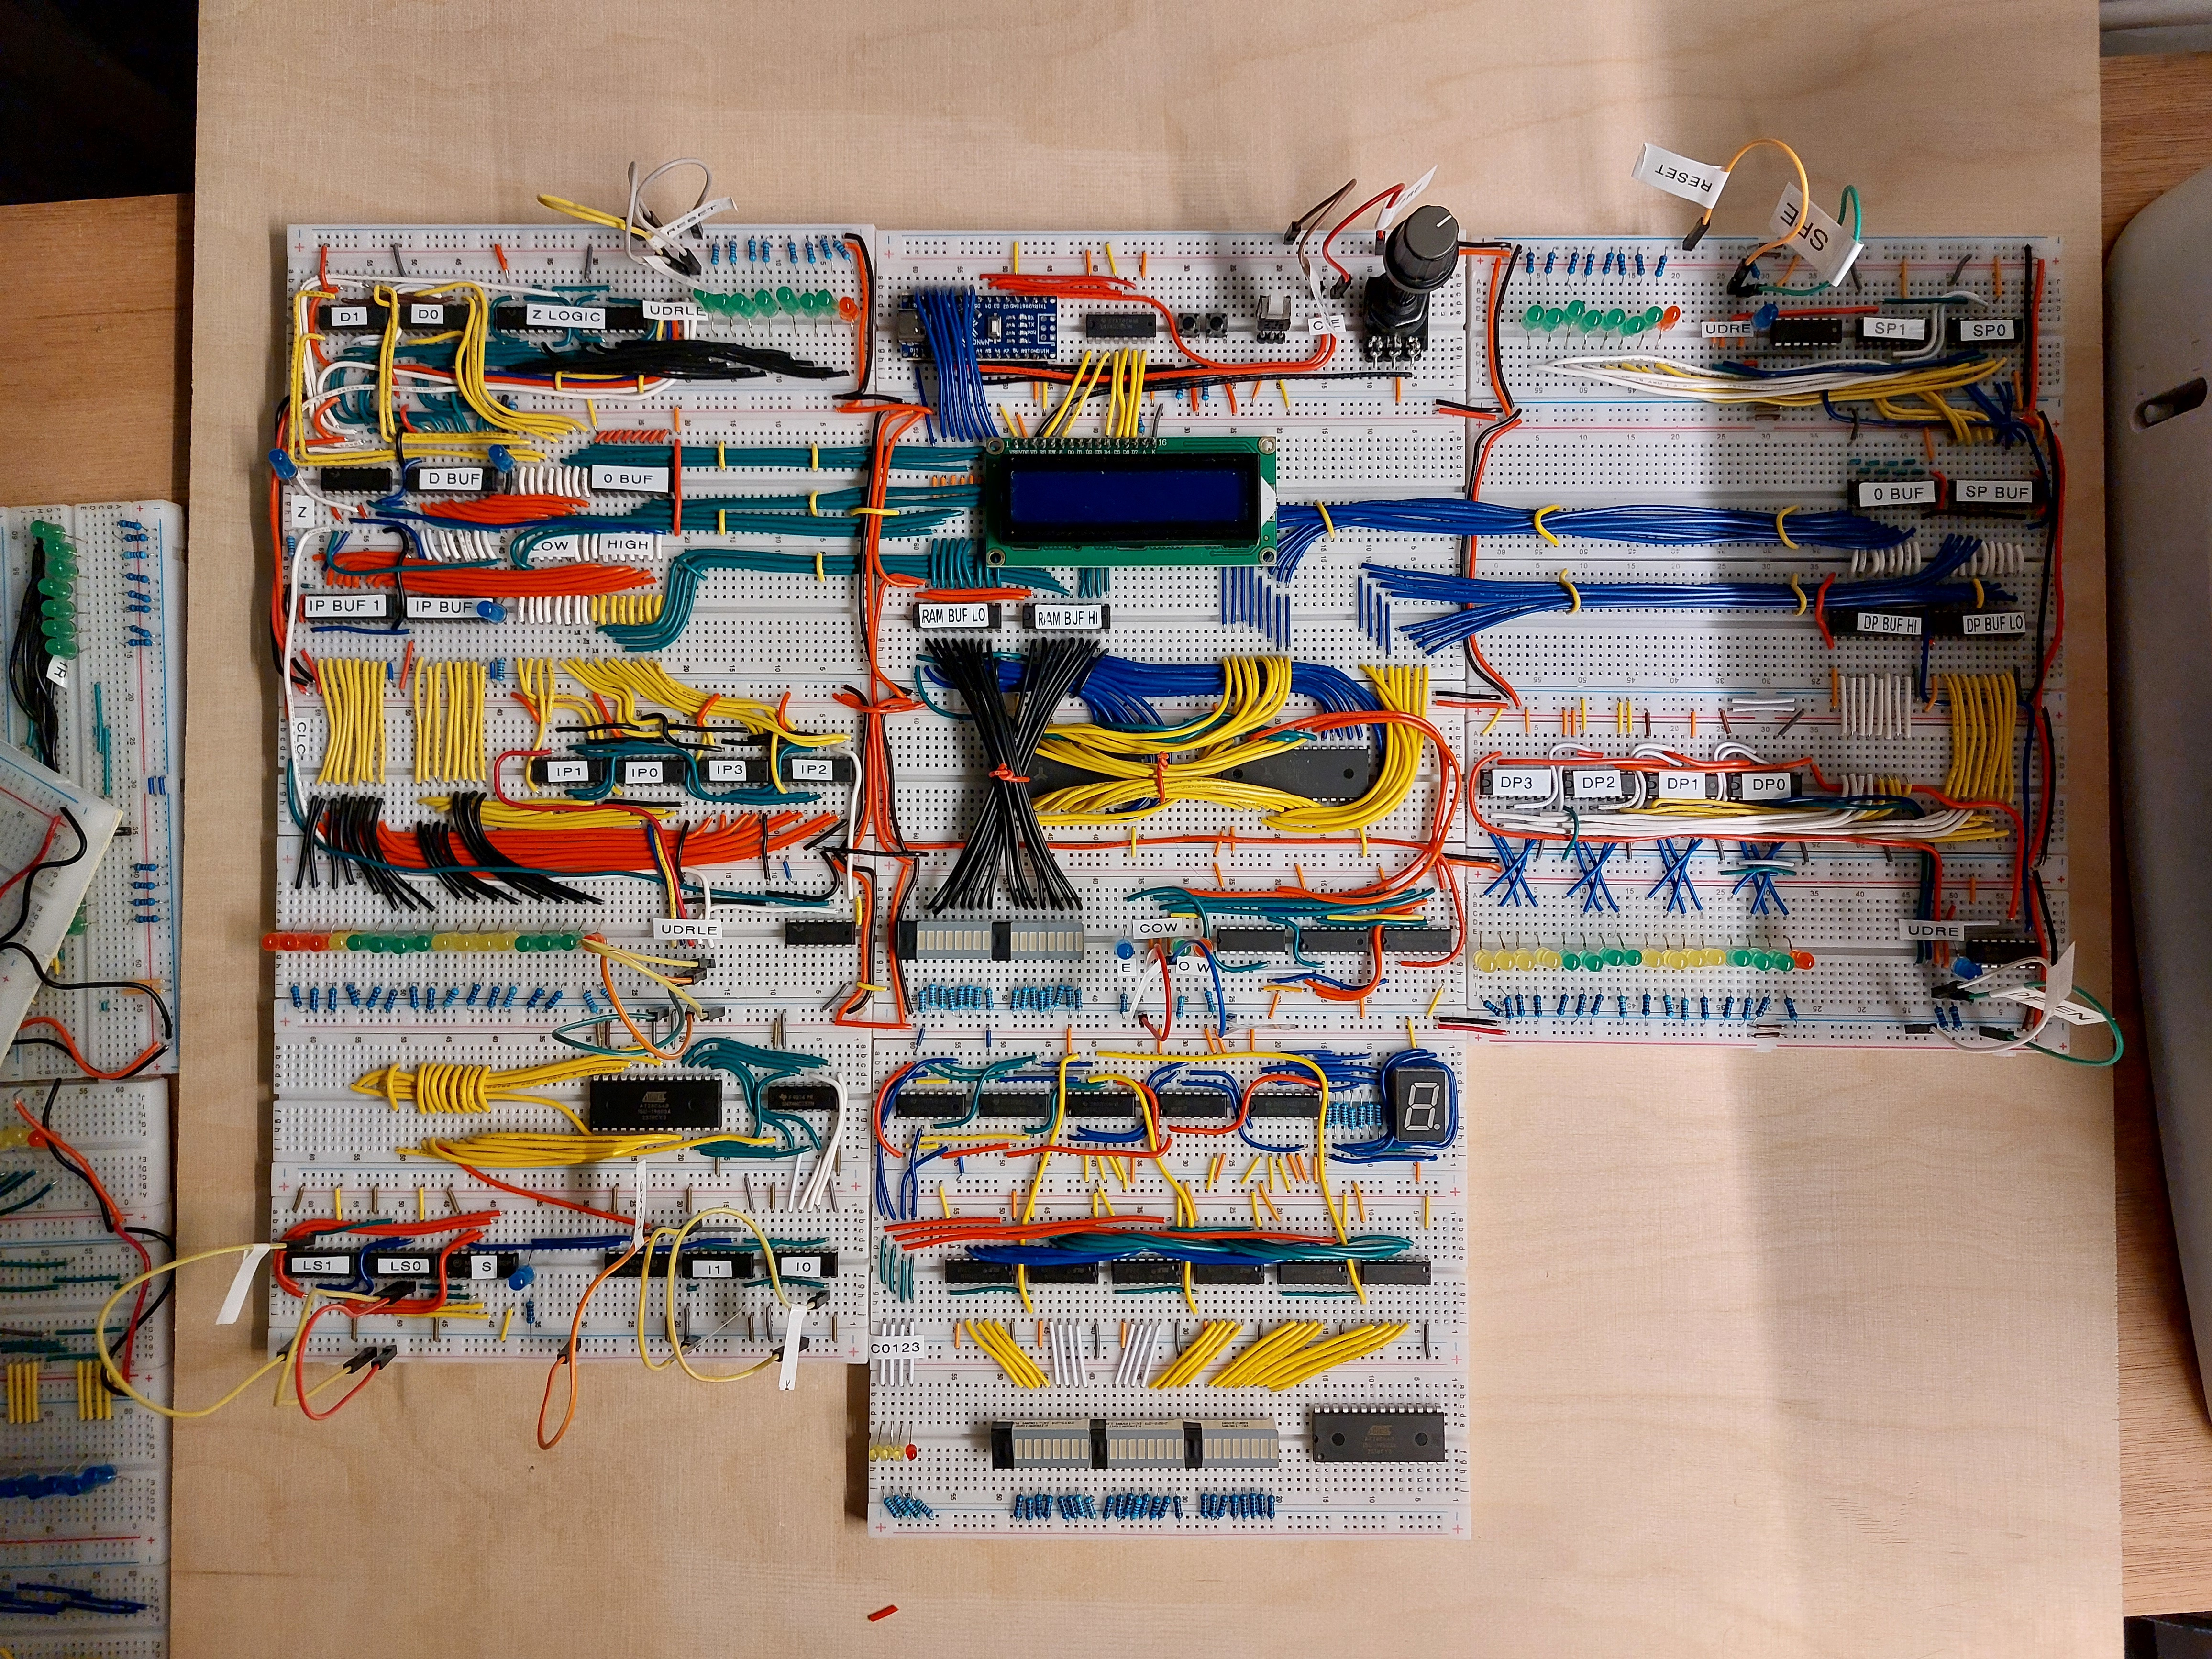
\includegraphics[height=.4\textheight]{img/pics/20241229_004603.jpg}
  \caption{The (segmented) control unit starts to take shape. The bottom-middle section contains the logic for sequentially fetching the three parts of the control-word sequentially from different sections in the MC EEPROM chip.}  
  \label{fig:earlybuild4}
\end{figure}
\vfill
\begin{figure}[H]
  \centering
  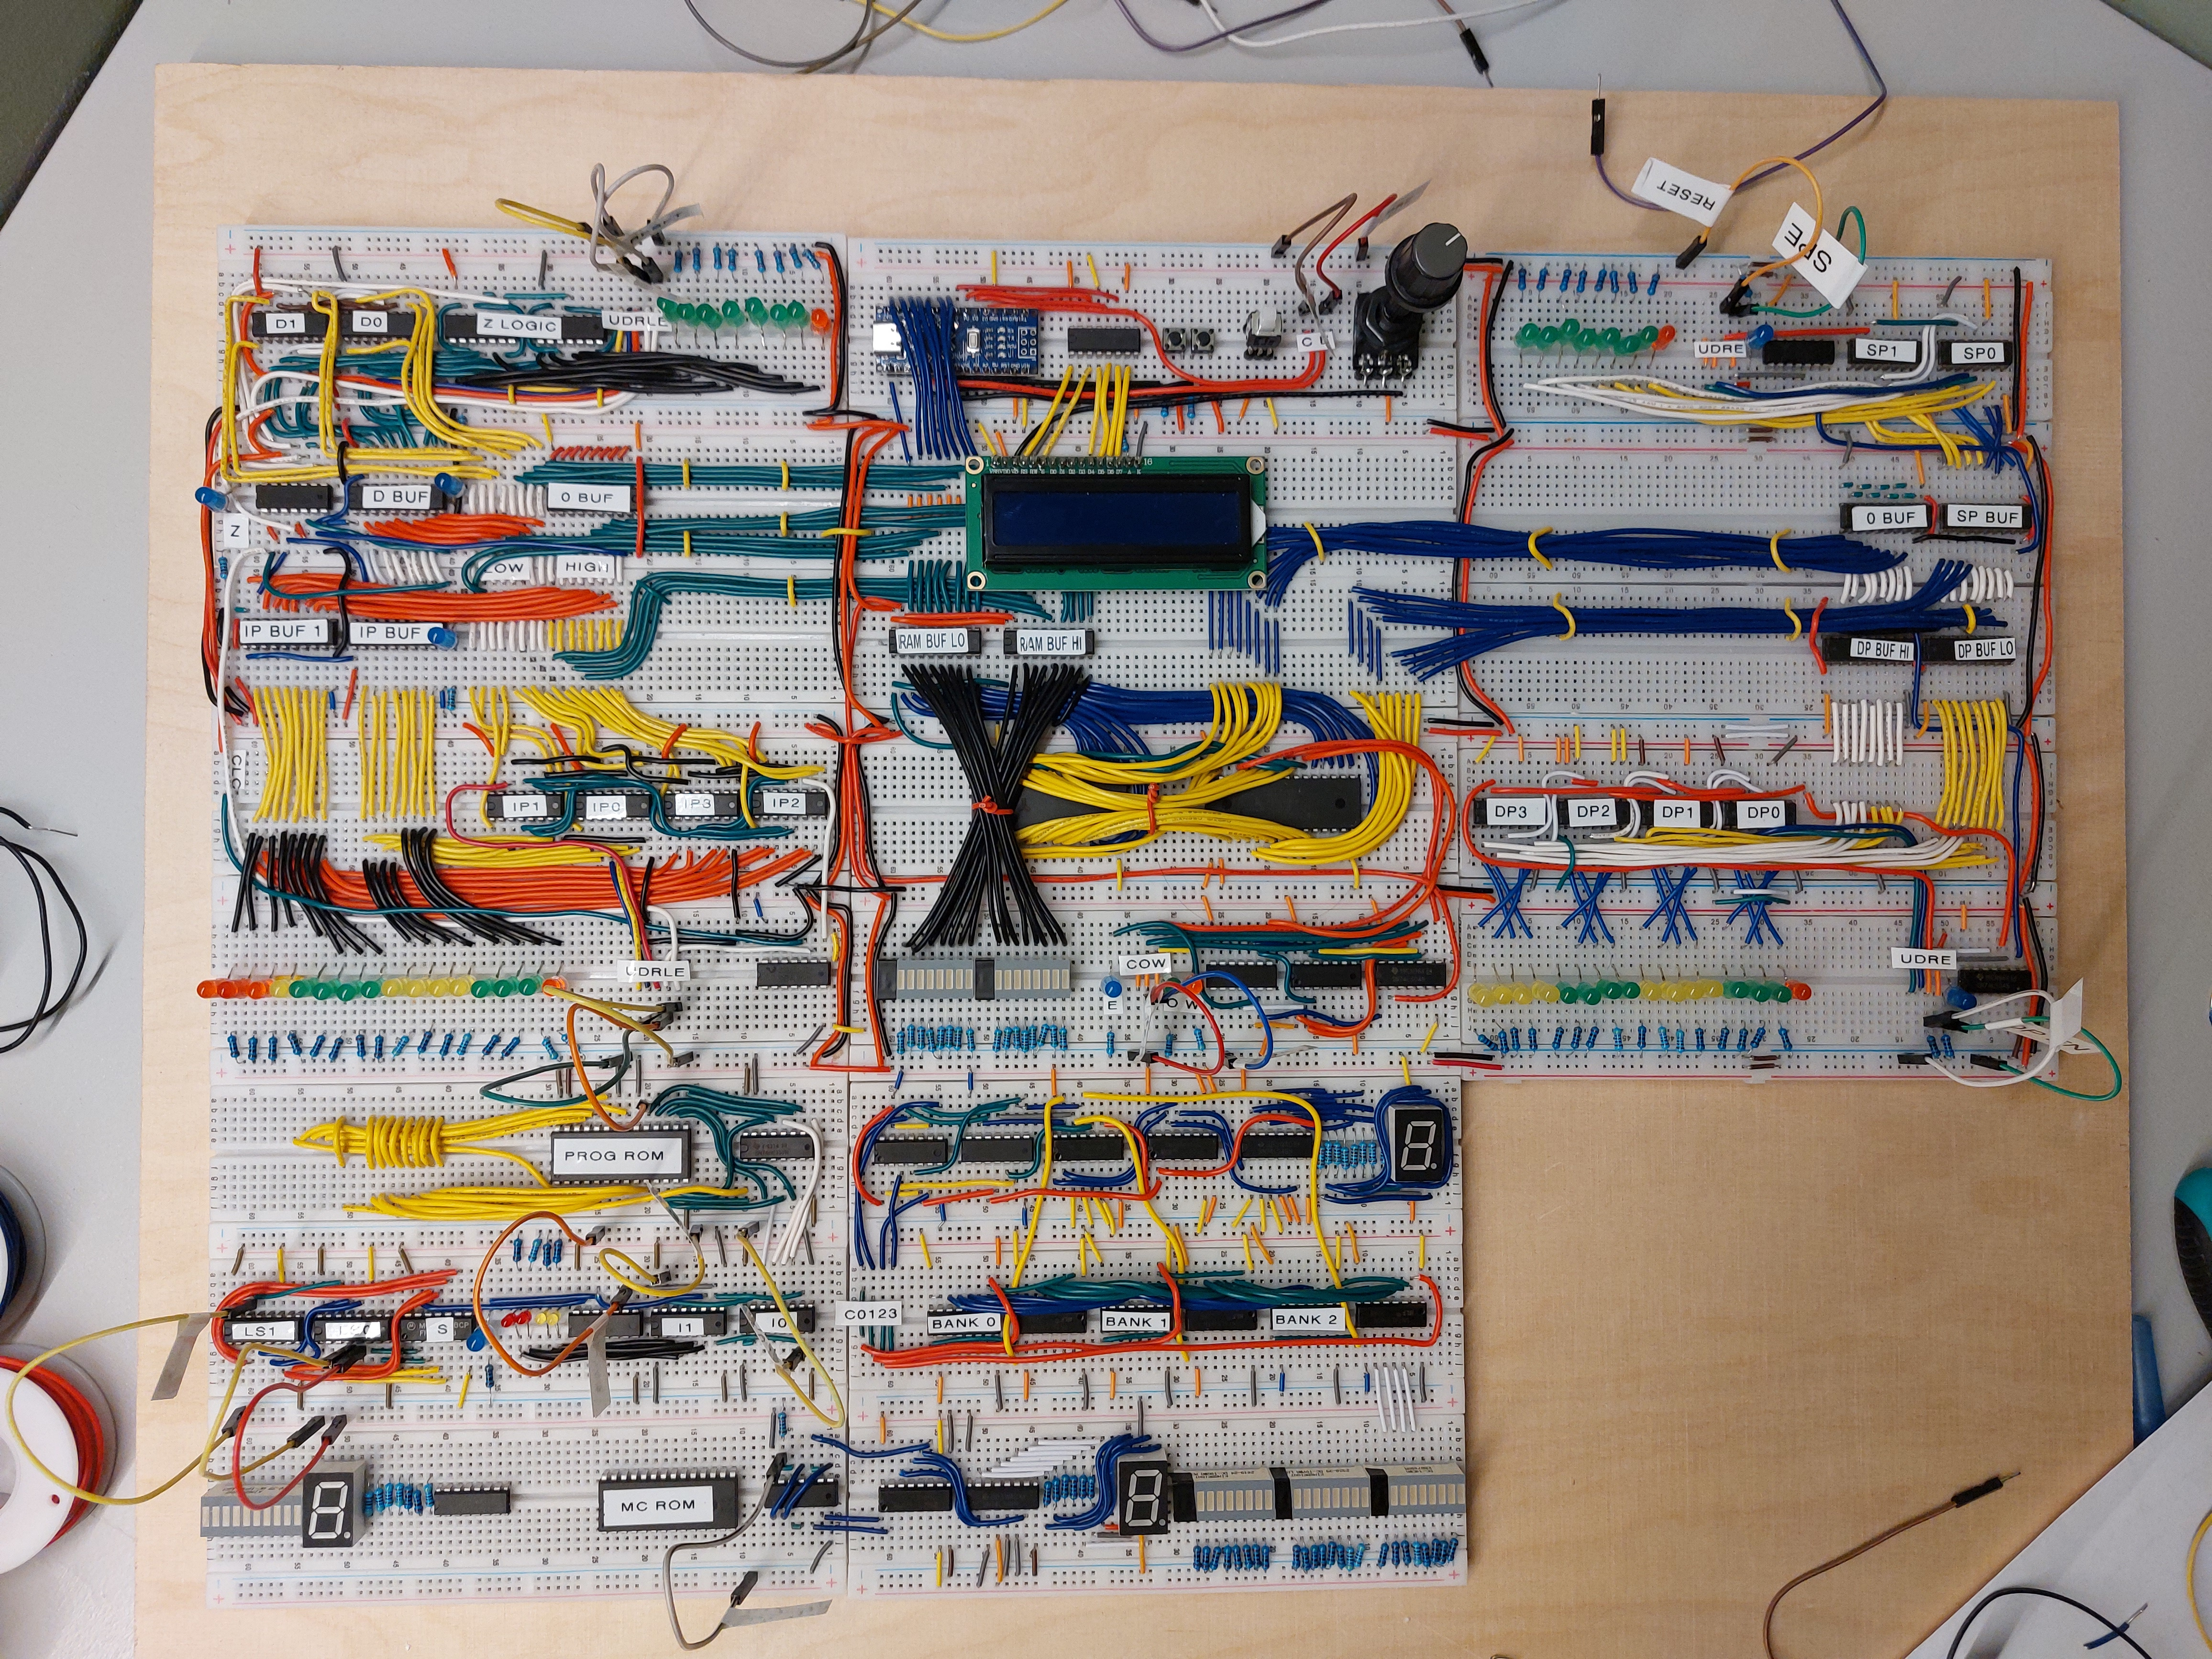
\includegraphics[height=.4\textheight]{img/pics/20241229_195125.jpg}
  \caption{The (segmented) control unit starts to take shape even more. A display for showing the current instrunction was added (7 segment display, bottom left).}
  \label{fig:earlybuild5}
\end{figure}
\vfill

\newpage

\vfill
\begin{figure}[H]
  \centering
  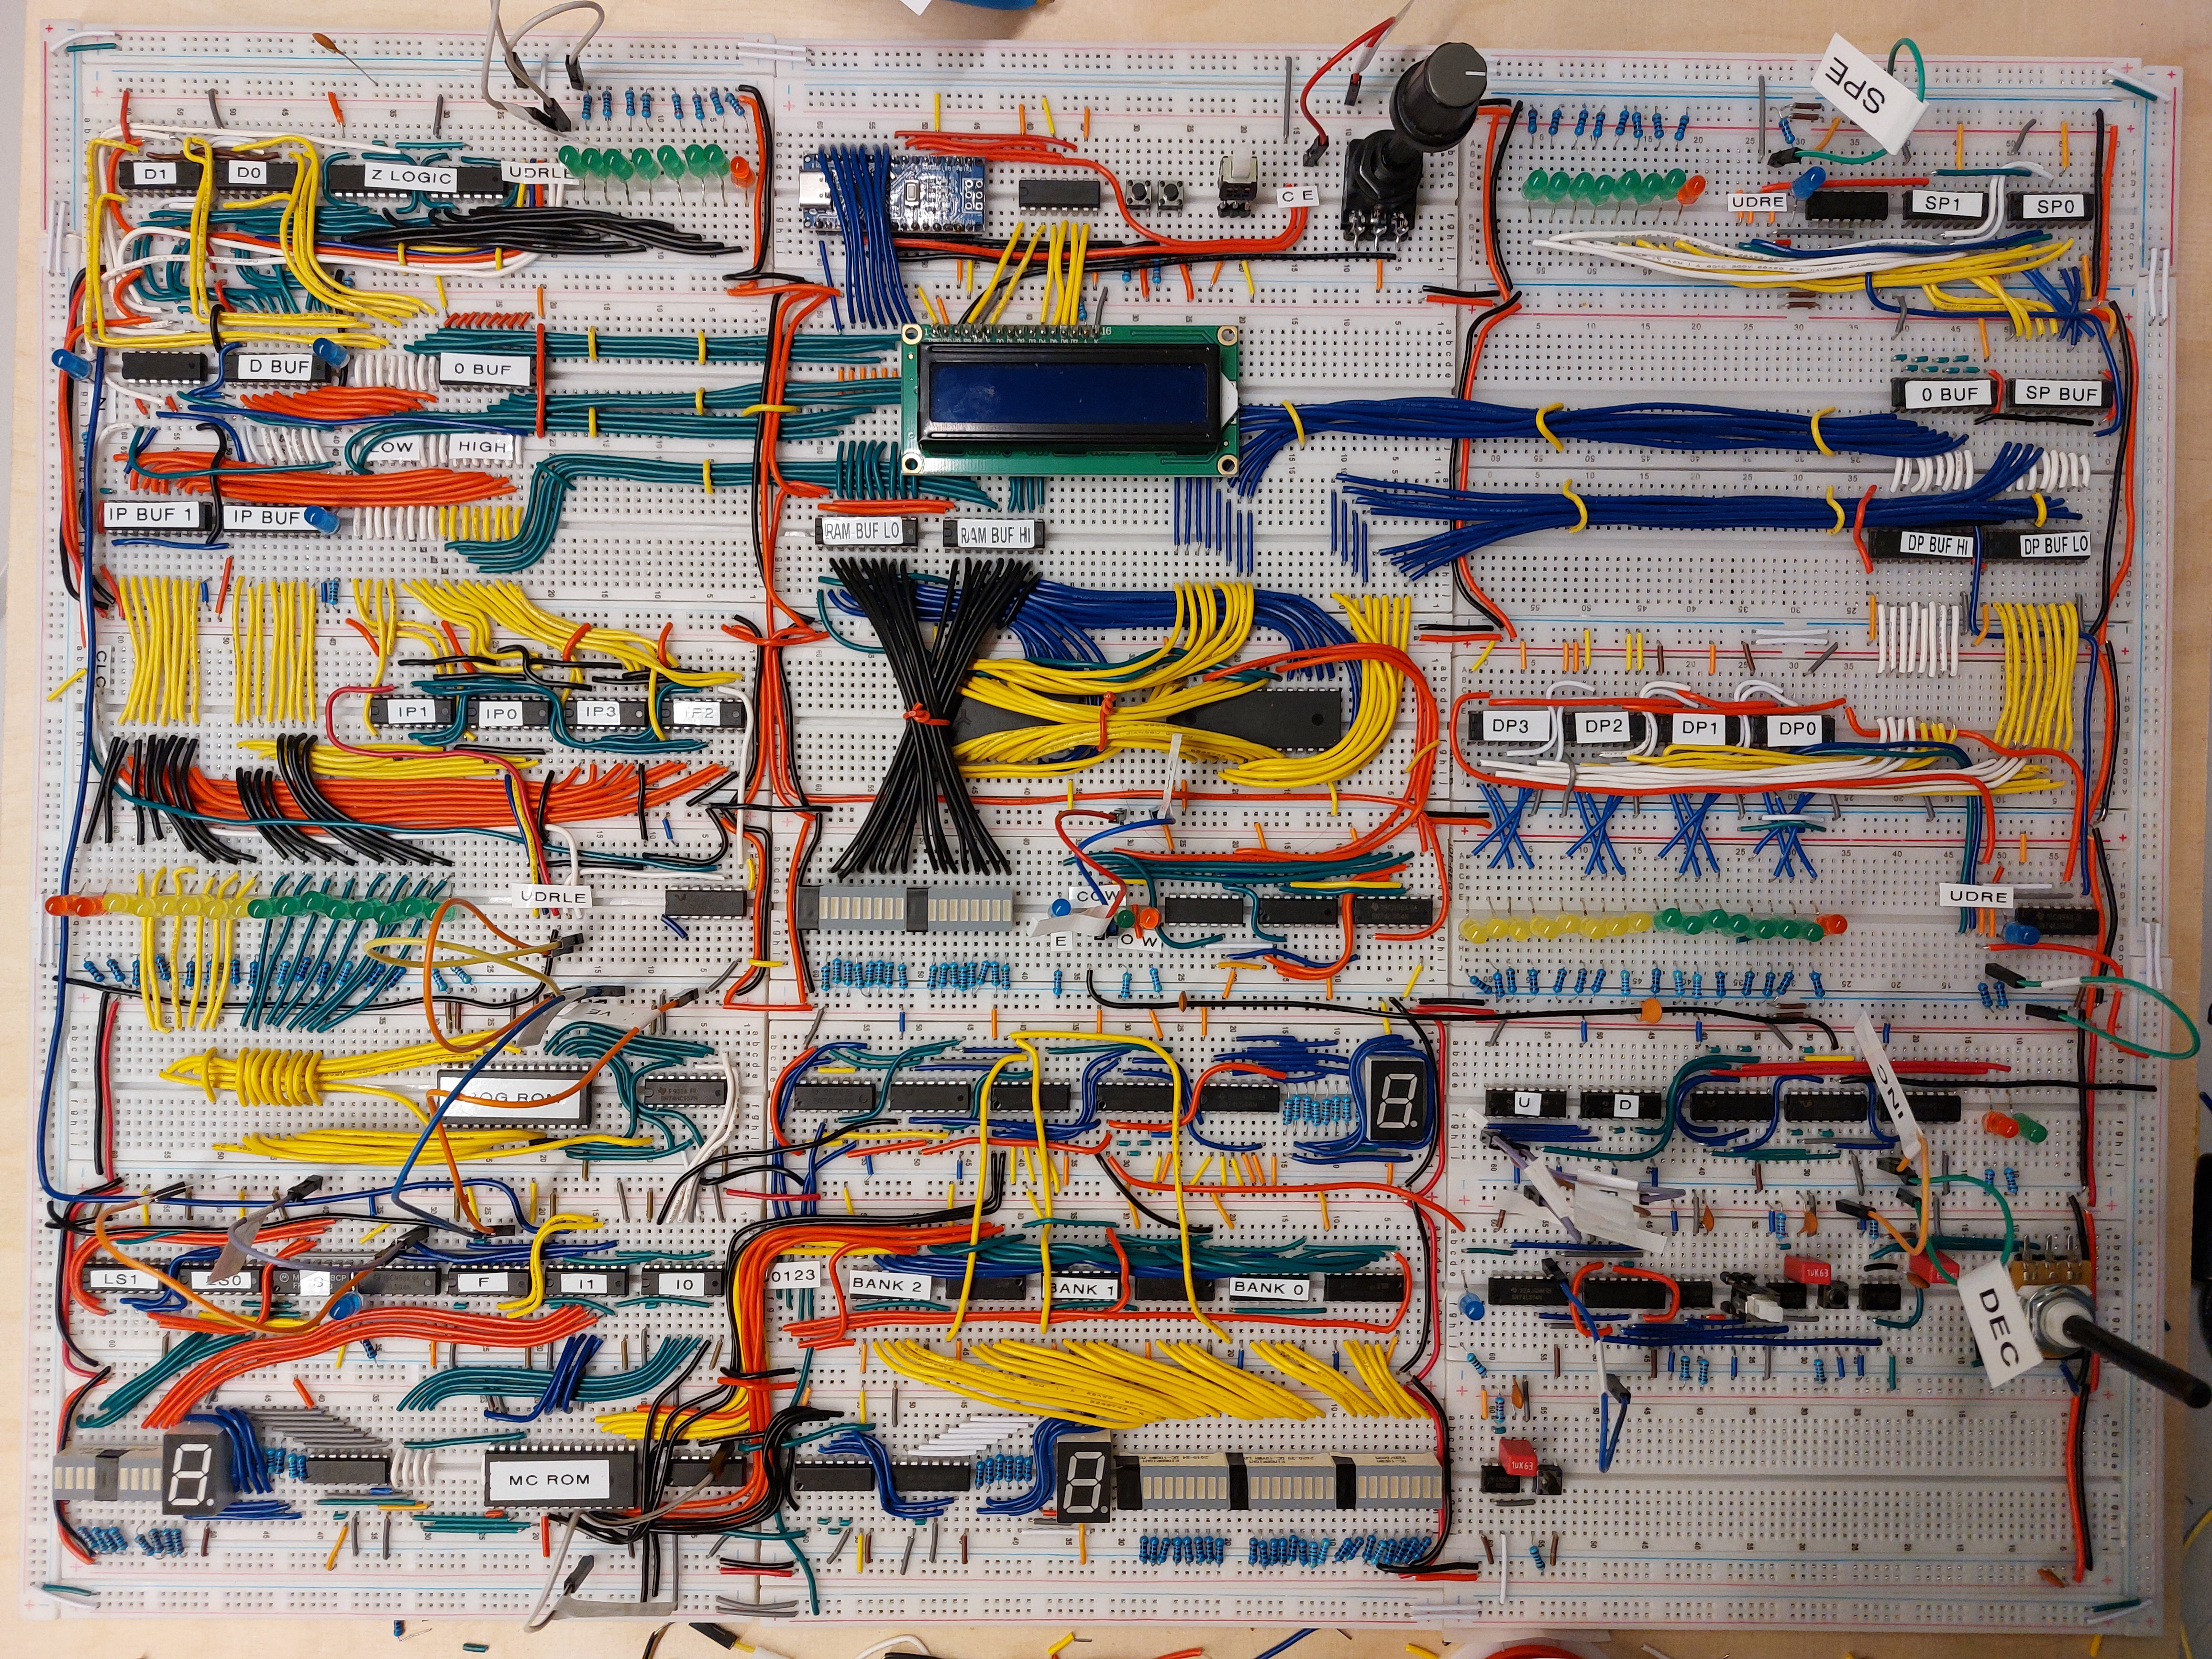
\includegraphics[height=.4\textheight]{img/pics/20250104_203015.jpg}
  \caption{First (somewhat) working version of the system.}
  \label{fig:firstbuild}
\end{figure}

\vfill
\begin{figure}[H]
  \centering
  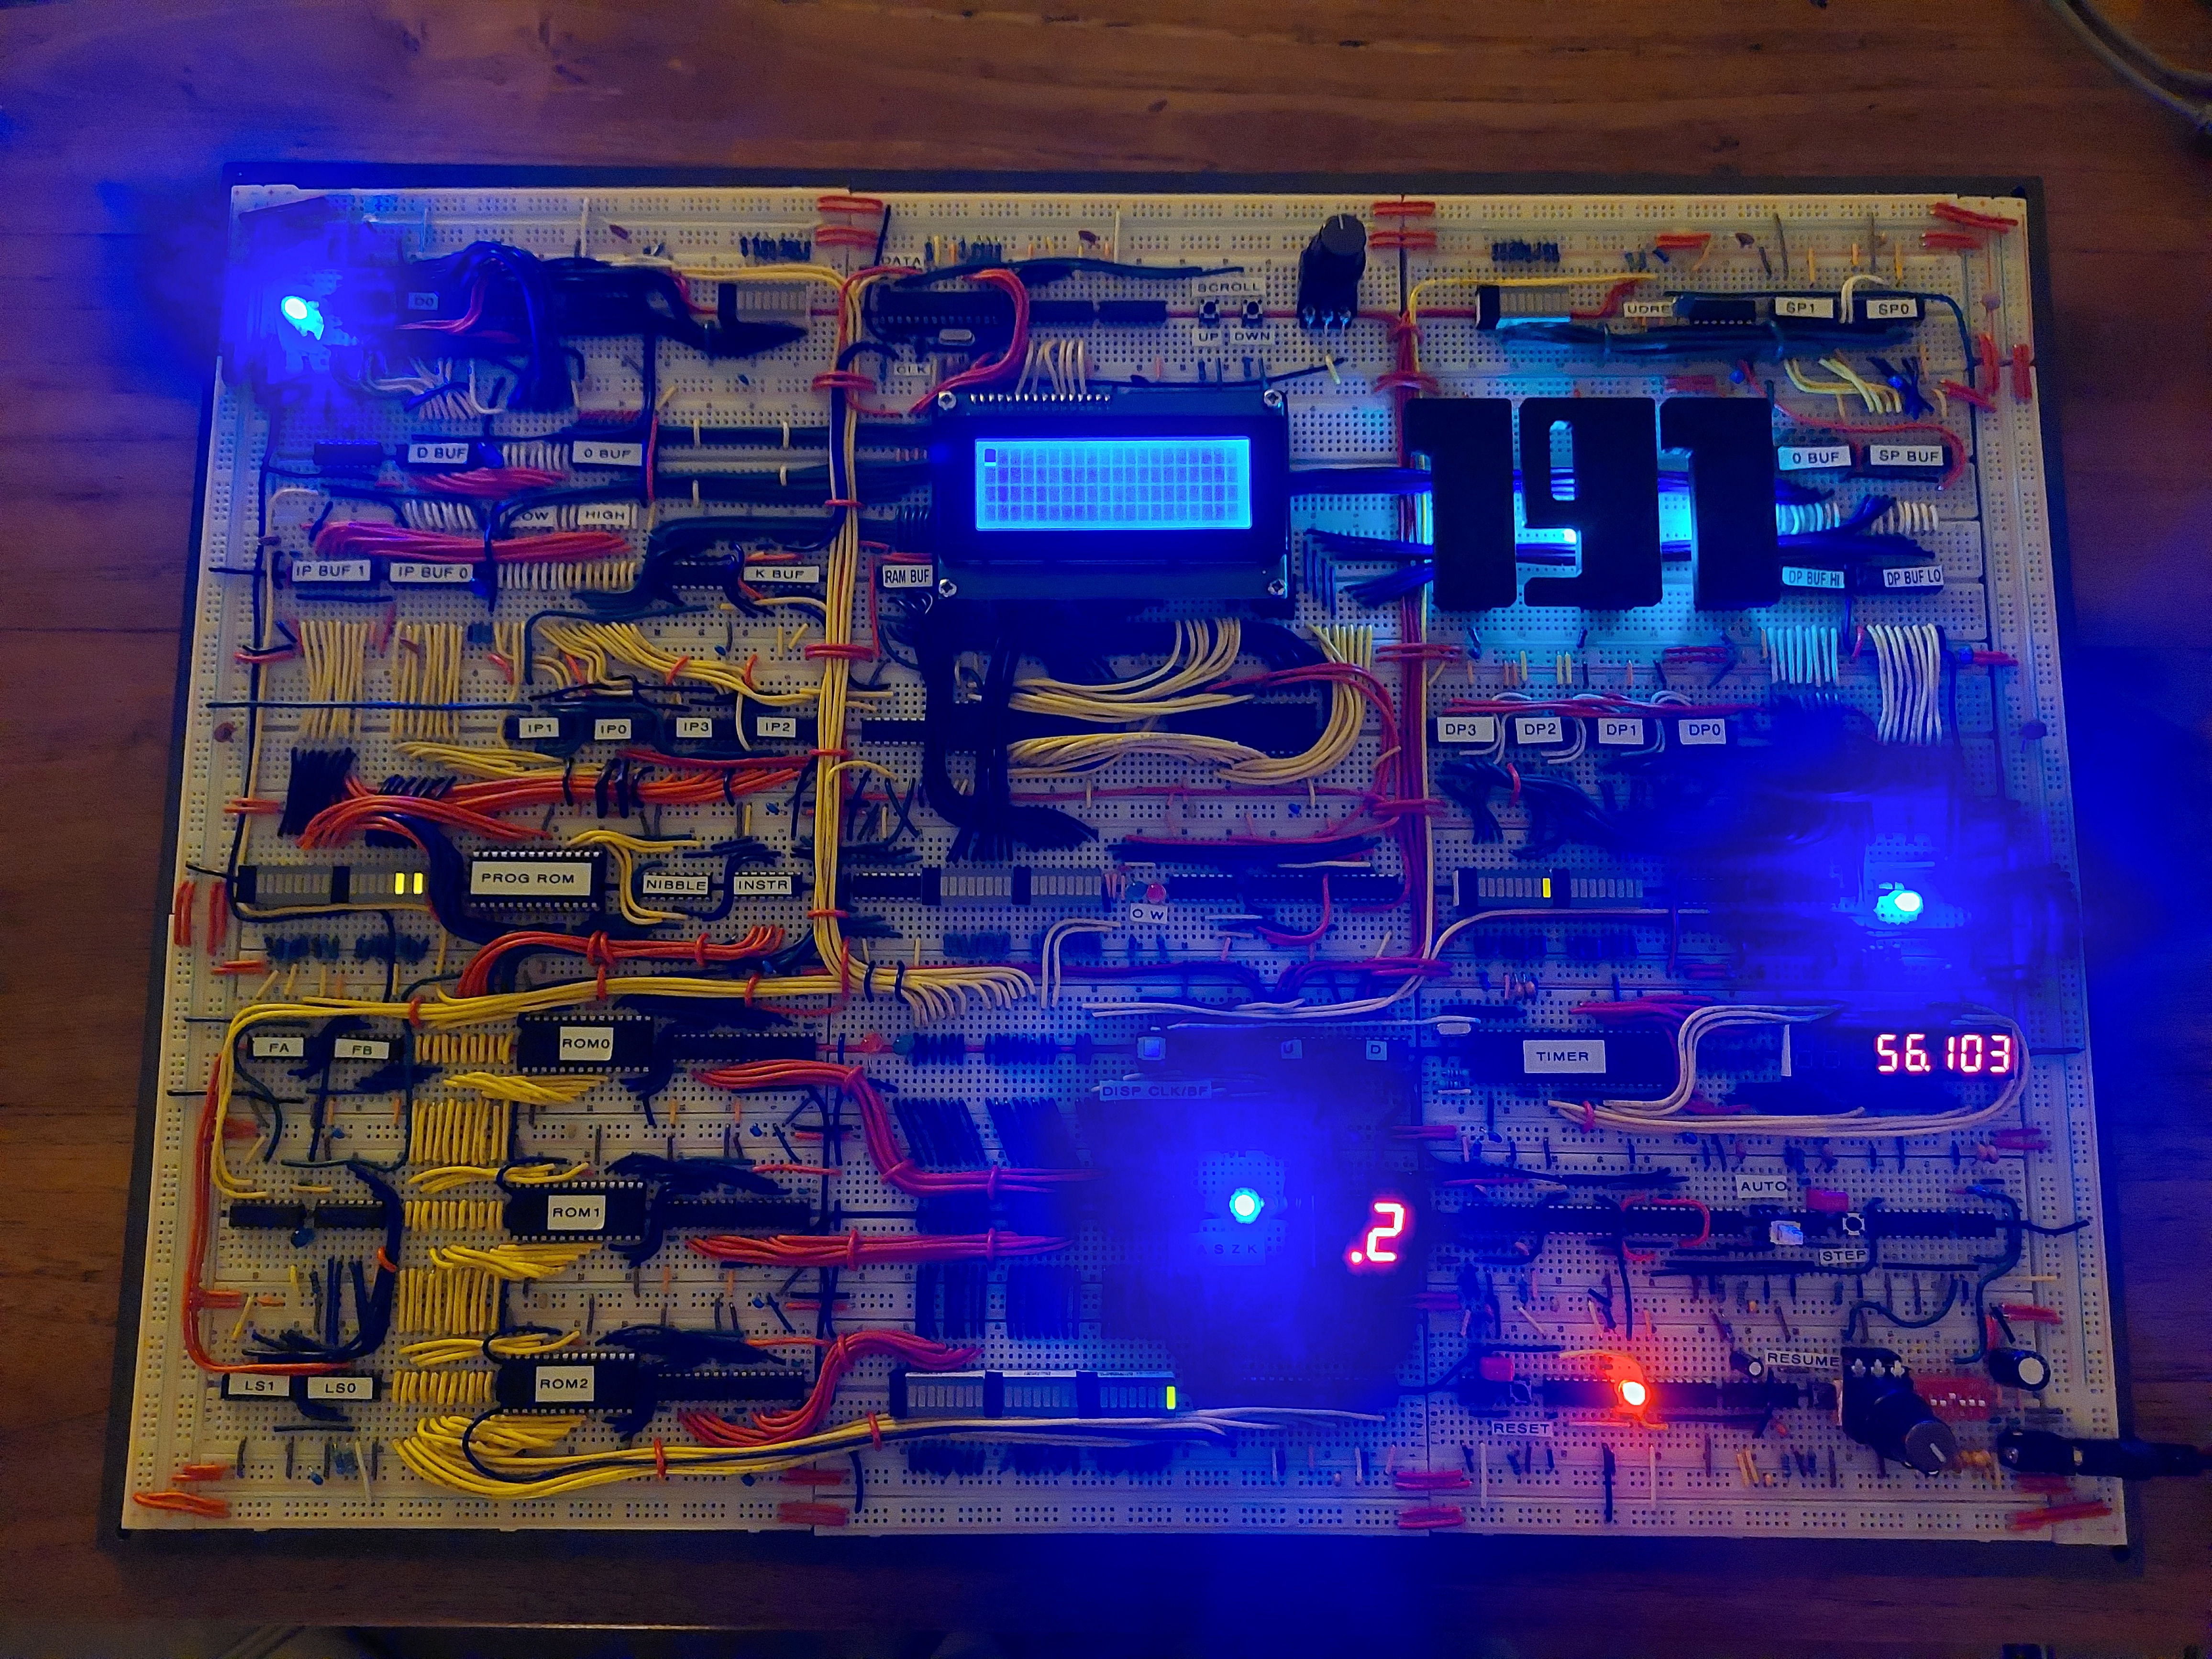
\includegraphics[height=.4\textheight]{img/pics/20251116_232655.jpg}
  \caption{Final build of the system, including 3D printed parts and many pretty lights.}
  \label{fig:finalbuild}
\end{figure}
\vfill
